\documentclass[a4paper, 12pt, oneside, titlepage]{article} %{\parskip}
\usepackage[top=2.54cm, bottom=2.54cm, left=3cm, right=2cm]{geometry}
\usepackage[utf8]{inputenc}
\usepackage[czech]{babel}
\usepackage[T1]{fontenc}
\usepackage{graphicx}
\usepackage{booktabs}
\usepackage{tabularx}
\usepackage{array}
\usepackage{indentfirst}
\usepackage{multicol}
\usepackage{titlesec}
\usepackage{mathtools}
\usepackage{esvect}

\usepackage{url}
\usepackage{caption}
\usepackage{subfig}
\usepackage[section]{placeins}
\usepackage{pdfpages}



\hyphenation{po-ly-gon desk-to-po-vá}

\newcommand{\tg}{\mathop{\rm tg}\nolimits}
\newcommand{\arctg}{\mathop{\rm arctg}\nolimits}
\newtheorem{defin}{Definice}

\begin{document}

%\pagestyle{empty}
\setcounter{page}{1}   % nastaví čítač stránek znovu od jedné
\pagenumbering{arabic} % číslování arabskými
\thispagestyle{empty}

\begin{center}

\large

\v{C}eské vysoké učení technické v~Praze

\medskip

Fakulta stavební
\medskip

Katedra geomatiky

\vfill
\centerline{\mbox{
\includegraphics[scale=1.3]{obrazky/symbol_cvut_konturova_verze.jpg}} }


{\bf\Large Technická zpráva}

\vfill

{\bf\LARGE\bfseries Algoritmy v digitální kartografii}

\vfill

{\bf\Large Úloha č. 4: Množinové operace s polygony}


\vfill



\vfill
\vspace{5mm}

\begin{tabular}{c}

{\bf Bc. Pane Kuzmanov}\\
\noalign{\vspace{2mm}}
{\bf Bc. František Mužík}\\
\noalign{\vspace{10mm}}

Studijní program: Geodézie a kartografie \\
\noalign{\vspace{2mm}}

Specializace: Geomatika\\

\end{tabular}


\vfill

% Zde doplňte rok
Praha 2021

\end{center}

%---------------------------------------------------------------------
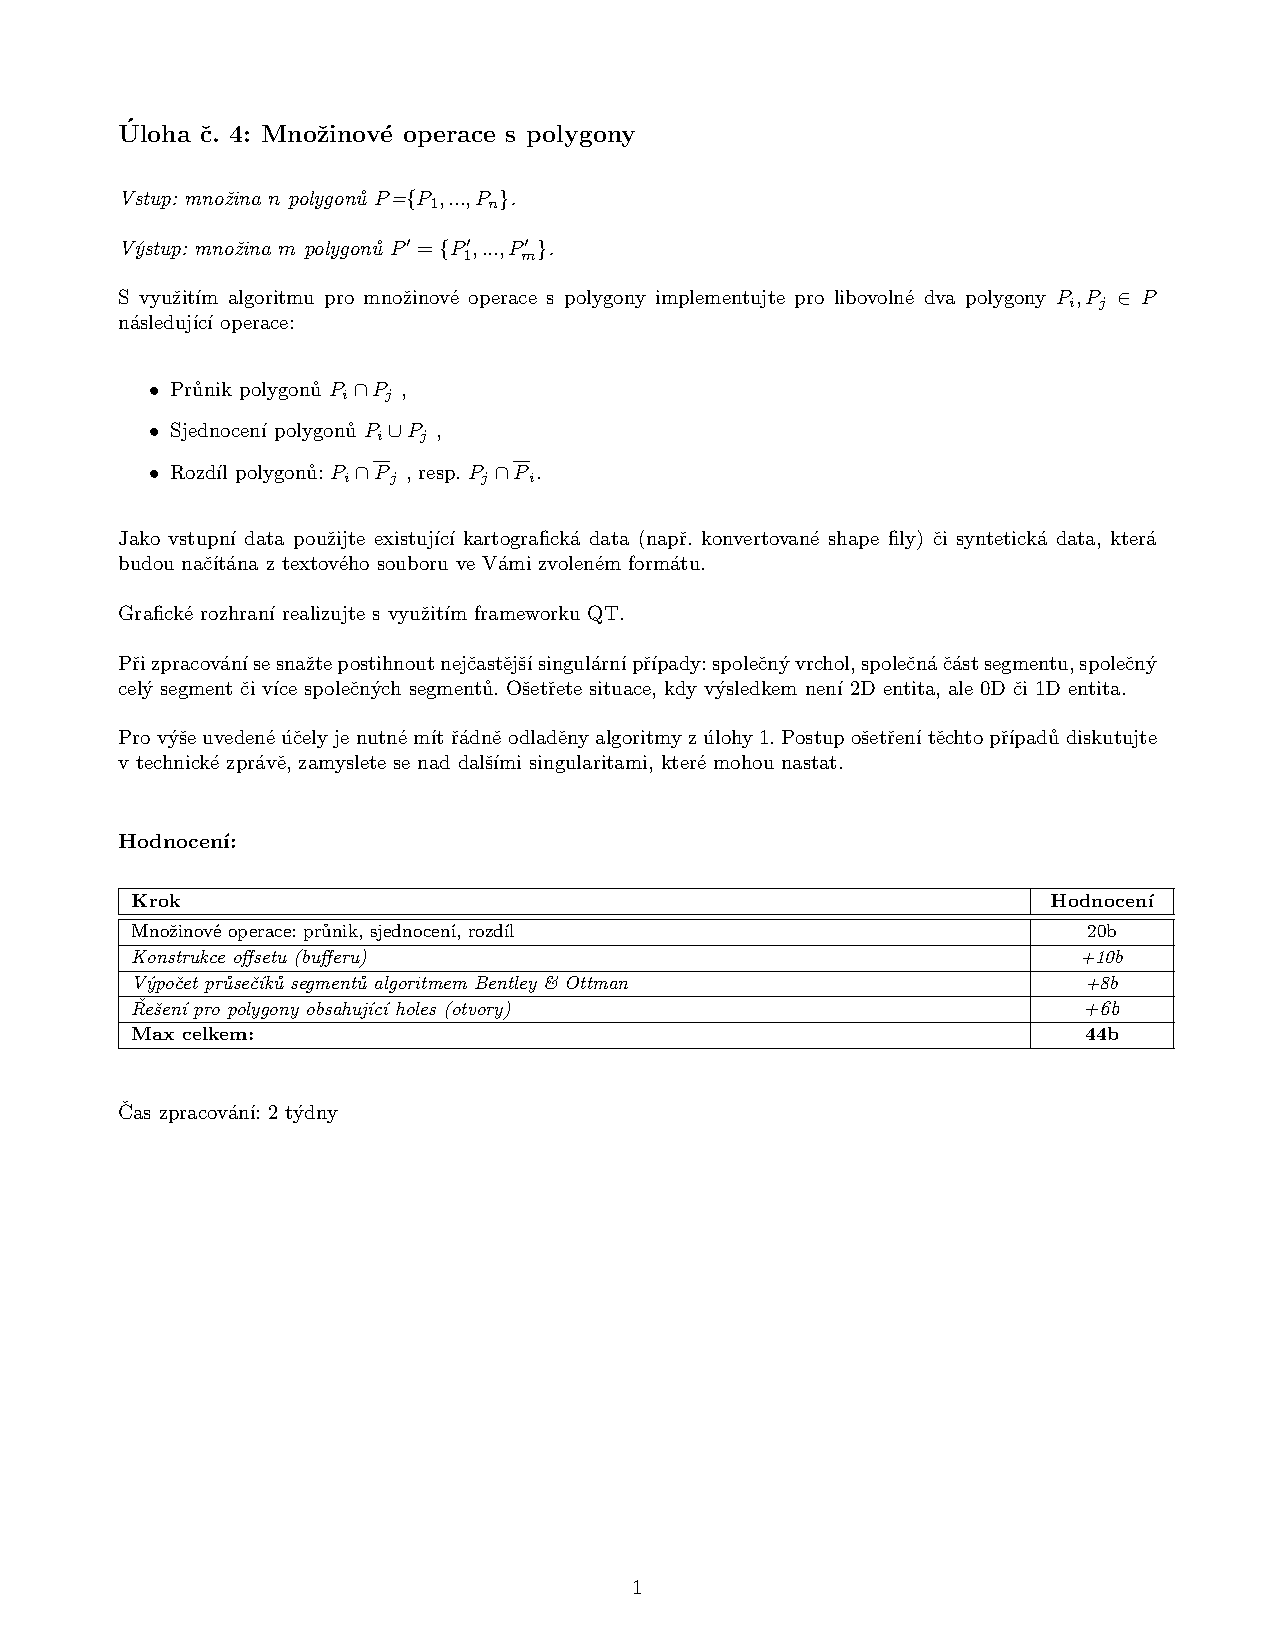
\includepdf{adkcv4}

%---------------------------------------------------------------------
\clearpage
\section{Údaje o bonusových úlohách}



\section{Popis a rozbor problému}



\section{Popisy algoritmů formálním jazykem} \label{popisalg}




\section{Vstupní data}
% formát vstupních dat, popis
ArcCR - kraje, chráněná území - Jihočeský kraj, NP+CHKO Šumava (Dissolve) - generalizace s tolerancí 1 km - feature vertices to point - přidání geometrie - table to excel


\section{Výstupní data}
% formát výstupních dat, popis



\section{Snímky obrazovky vytvořené aplikace a její popis}\label{snimky}




\section{Dokumentace}
% popis tříd, datových položek a jednotlivých metod


\section{Závěr}
 Vývoj aplikace proběhl v~programovacím jazyce C++. 

\subsection{Možné či neřešené problémy} \label{mcn_problemy}

\subsection{Náměty na vylepšení} \label{vylepseni}





\begin{flushright}
V Praze 27. 12.2021\\
\vspace{2mm}
Bc. Pane Kuzmanov\\
Bc. František Mužík\\
\end{flushright}


%---------------------------------------------------------------------
\clearpage 
\section*{Použitá literatura}
\renewcommand{\section}[2]{}%
\bibliographystyle{acm}
\bibliography{Literatura_u4_adk}


\end{document}
